% Important: If latex complains about unicode characters,
% please use "\usepackage[utf8x]{inputenc}" in your preamble
% You can change the size of the picture by putting it into the construct:
% 1) \resizebox{10cm}{!}{"below picture"} to scale horizontally to 10 cm
% 2) \resizebox{!}{15cm}{"below picture"} to scale vertically to 15 cm
% 3) \resizebox{10cm}{15cm}{"below picture"} a combination of above two
% It is not recomended to use the scale option of the tikzpicture environment.
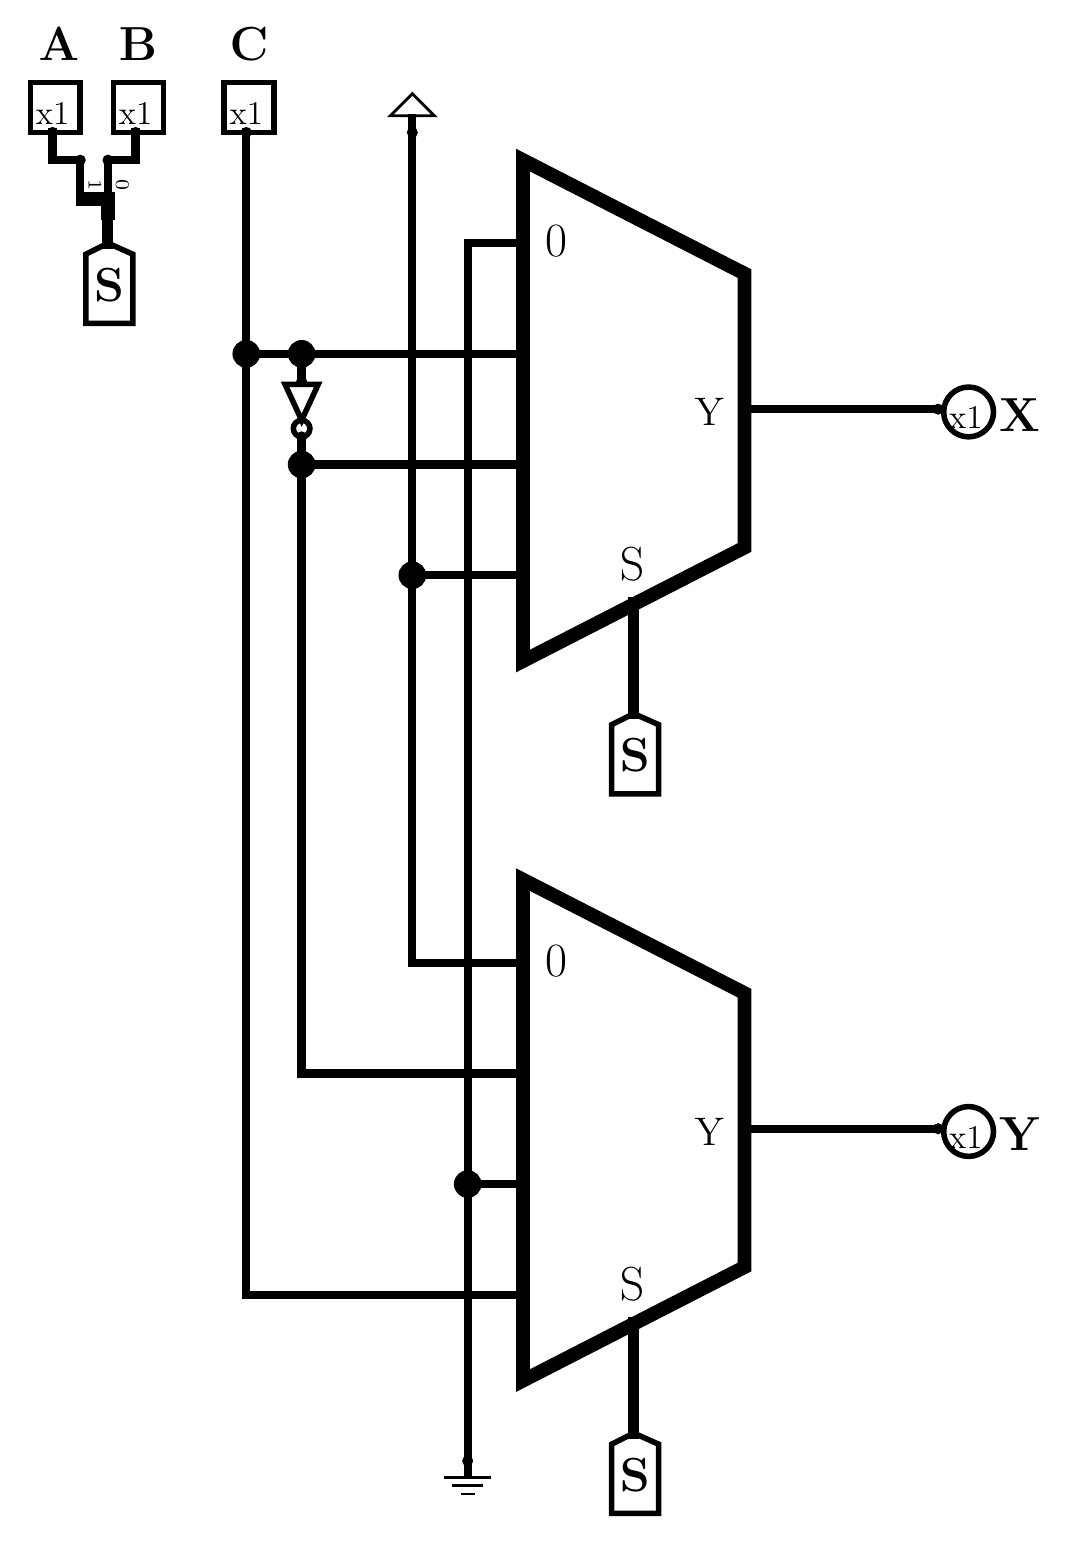
\begin{tikzpicture}[x=1pt,y=-1pt,line cap=rect]
\def\logisimfontA#1{\fontfamily{cmr}{#1}} % Replaced by logisim, original font was "SansSerif"
\def\logisimfontB#1{\fontfamily{CMU Sans Serif}{#1}}
\def\logisimfontC#1{\fontfamily{Ubuntu}{#1}}
\definecolor{custcol_0_0_0}{RGB}{0, 0, 0}
\definecolor{custcol_ff_ff_ff}{RGB}{255, 255, 255}
\draw [line width=4.0pt, custcol_0_0_0 ]  (35.0,78.0) -- (35.0,88.0) ;
\draw [line width=3.0pt, custcol_0_0_0 ]  (185.0,208.0) -- (145.0,208.0) -- (145.0,348.0) -- (185.0,348.0) ;
\draw [line width=3.0pt, custcol_0_0_0 ]  (85.0,48.0) -- (85.0,128.0) -- (85.0,468.0) -- (185.0,468.0) ;
\draw [line width=4.0pt, custcol_0_0_0 ]  (225.0,218.0) -- (225.0,258.0) ;
\draw [line width=4.0pt, custcol_0_0_0 ]  (225.0,478.0) -- (225.0,518.0) ;
\draw [line width=3.0pt, custcol_0_0_0 ]  (85.0,128.0) -- (105.0,128.0) -- (105.0,138.0) ;
\draw [line width=3.0pt, custcol_0_0_0 ]  (165.0,428.0) -- (185.0,428.0) ;
\draw [line width=3.0pt, custcol_0_0_0 ]  (105.0,168.0) -- (185.0,168.0) ;
\draw [line width=3.0pt, custcol_0_0_0 ]  (105.0,128.0) -- (185.0,128.0) ;
\draw [line width=3.0pt, custcol_0_0_0 ]  (105.0,158.0) -- (105.0,168.0) -- (105.0,388.0) -- (185.0,388.0) ;
\draw [line width=3.0pt, custcol_0_0_0 ]  (265.0,148.0) -- (335.0,148.0) ;
\draw [line width=3.0pt, custcol_0_0_0 ]  (265.0,408.0) -- (335.0,408.0) ;
\fill [line width=3.0pt, custcol_0_0_0]  (105.0,128.0) ellipse (5.0 and 5.0 );
\fill [line width=3.0pt, custcol_0_0_0]  (85.0,128.0) ellipse (5.0 and 5.0 );
\fill [line width=3.0pt, custcol_0_0_0]  (145.0,208.0) ellipse (5.0 and 5.0 );
\fill [line width=3.0pt, custcol_0_0_0]  (105.0,168.0) ellipse (5.0 and 5.0 );
\fill [line width=3.0pt, custcol_0_0_0]  (165.0,428.0) ellipse (5.0 and 5.0 );
\logisimfontB{\fontsize{14pt}{14pt}\fontseries{bx}\selectfont\node[inner sep=0, outer sep=0, custcol_0_0_0, anchor=base west] at  (247.0,154.0)  {Y};}
\draw [line width=5.0pt, custcol_0_0_0 ]  (185.0,58.0) -- (185.0,239.0) -- (265.0,198.0) -- (265.0,99.0) -- cycle;
\logisimfontB{\fontsize{16pt}{16pt}\fontseries{bx}\selectfont\node[inner sep=0, outer sep=0, custcol_0_0_0, anchor=base west] at  (193.0,93.0)  {0};}
\logisimfontC{\fontsize{16pt}{16pt}\fontseries{bx}\selectfont\node[inner sep=0, outer sep=0, custcol_0_0_0, anchor=base west] at  (220.0,210.0)  {S};}
\fill [line width=1.0pt, custcol_0_0_0]  (185.0,88.0) ellipse (2.0 and 2.0 );
\fill [line width=1.0pt, custcol_0_0_0]  (185.0,128.0) ellipse (2.0 and 2.0 );
\fill [line width=1.0pt, custcol_0_0_0]  (185.0,168.0) ellipse (2.0 and 2.0 );
\fill [line width=1.0pt, custcol_0_0_0]  (185.0,208.0) ellipse (2.0 and 2.0 );
\fill [line width=1.0pt, custcol_0_0_0]  (225.0,218.0) ellipse (2.0 and 2.0 );
\fill [line width=1.0pt, custcol_0_0_0]  (265.0,148.0) ellipse (2.0 and 2.0 );
\logisimfontB{\fontsize{14pt}{14pt}\fontseries{bx}\selectfont\node[inner sep=0, outer sep=0, custcol_0_0_0, anchor=base west] at  (247.0,414.0)  {Y};}
\draw [line width=5.0pt, custcol_0_0_0 ]  (185.0,318.0) -- (185.0,499.0) -- (265.0,458.0) -- (265.0,359.0) -- cycle;
\logisimfontB{\fontsize{16pt}{16pt}\fontseries{bx}\selectfont\node[inner sep=0, outer sep=0, custcol_0_0_0, anchor=base west] at  (193.0,353.0)  {0};}
\logisimfontC{\fontsize{16pt}{16pt}\fontseries{bx}\selectfont\node[inner sep=0, outer sep=0, custcol_0_0_0, anchor=base west] at  (220.0,470.0)  {S};}
\fill [line width=1.0pt, custcol_0_0_0]  (185.0,348.0) ellipse (2.0 and 2.0 );
\fill [line width=1.0pt, custcol_0_0_0]  (185.0,388.0) ellipse (2.0 and 2.0 );
\fill [line width=1.0pt, custcol_0_0_0]  (185.0,428.0) ellipse (2.0 and 2.0 );
\fill [line width=1.0pt, custcol_0_0_0]  (185.0,468.0) ellipse (2.0 and 2.0 );
\fill [line width=1.0pt, custcol_0_0_0]  (225.0,478.0) ellipse (2.0 and 2.0 );
\fill [line width=1.0pt, custcol_0_0_0]  (265.0,408.0) ellipse (2.0 and 2.0 );
\draw [line width=3.0pt, custcol_0_0_0 ]  (185.0,88.0) -- (165.0,88.0) -- (165.0,428.0) -- (165.0,528.0) -- (165.0,533.0) ;
\draw [line width=1.0pt, custcol_0_0_0 ]  (173.0,534.0) -- (157.0,534.0) ;
\draw [line width=1.0pt, custcol_0_0_0 ]  (170.0,537.0) -- (160.0,537.0) ;
\draw [line width=1.0pt, custcol_0_0_0 ]  (167.0,540.0) -- (163.0,540.0) ;
\fill [line width=1.0pt, custcol_0_0_0]  (165.0,528.0) ellipse (2.0 and 2.0 );
\draw [line width=2.0pt, custcol_0_0_0 ]  (105.0,152.0) -- (111.0,139.0) -- (99.0,139.0) -- cycle;
\draw [line width=2.0pt, custcol_0_0_0, rotate around={-270: (105.0,155.0) }]  (105.0,155.0) ellipse (3.0 and 3.0 );
\fill [line width=2.0pt, custcol_0_0_0]  (105.0,158.0) ellipse (2.0 and 2.0 );
\fill [line width=2.0pt, custcol_0_0_0]  (105.0,138.0) ellipse (2.0 and 2.0 );
\draw [line width=2.0pt, custcol_0_0_0]  (346.0,149.0) ellipse (9.0 and 9.0 );
\logisimfontA{\fontsize{12pt}{12pt}\selectfont\node[inner sep=0, outer sep=0, custcol_0_0_0, anchor=base west] at  (339.0,155.0)  {x1};}
\logisimfontA{\fontsize{16pt}{16pt}\fontseries{bx}\selectfont\node[inner sep=0, outer sep=0, custcol_0_0_0, anchor=base west] at  (357.0,156.0)  {X};}
\fill [line width=2.0pt, custcol_0_0_0]  (335.0,148.0) ellipse (2.0 and 2.0 );
\draw [line width=2.0pt, custcol_0_0_0]  (346.0,409.0) ellipse (9.0 and 9.0 );
\logisimfontA{\fontsize{12pt}{12pt}\selectfont\node[inner sep=0, outer sep=0, custcol_0_0_0, anchor=base west] at  (339.0,415.0)  {x1};}
\logisimfontA{\fontsize{16pt}{16pt}\fontseries{bx}\selectfont\node[inner sep=0, outer sep=0, custcol_0_0_0, anchor=base west] at  (357.0,416.0)  {Y};}
\fill [line width=2.0pt, custcol_0_0_0]  (335.0,408.0) ellipse (2.0 and 2.0 );
\draw [line width=3.0pt, custcol_0_0_0 ]  (145.0,208.0) -- (145.0,48.0) -- (145.0,43.0) ;
\draw [line width=1.0pt, custcol_0_0_0 ]  (137.0,42.0) -- (145.0,34.0) -- (153.0,42.0) -- cycle;
\fill [line width=1.0pt, custcol_0_0_0]  (145.0,48.0) ellipse (2.0 and 2.0 );
\draw [line width=2.0pt, custcol_0_0_0 ]  (77.0,30.0) -- (94.0,30.0) ;
\draw [line width=2.0pt, custcol_0_0_0 ]  (95.0,30.0) -- (95.0,47.0) ;
\draw [line width=2.0pt, custcol_0_0_0 ]  (95.0,48.0) -- (78.0,48.0) ;
\draw [line width=2.0pt, custcol_0_0_0 ]  (77.0,48.0) -- (77.0,31.0) ;
\logisimfontA{\fontsize{12pt}{12pt}\selectfont\node[inner sep=0, outer sep=0, custcol_0_0_0, anchor=base west] at  (79.0,45.0)  {x1};}
\logisimfontA{\fontsize{16pt}{16pt}\fontseries{bx}\selectfont\node[inner sep=0, outer sep=0, custcol_0_0_0, anchor=base west] at  (79.0,22.0)  {C};}
\fill [line width=2.0pt, custcol_0_0_0]  (85.0,48.0) ellipse (2.0 and 2.0 );
\draw [line width=2.0pt, custcol_0_0_0 ]  (7.0,30.0) -- (24.0,30.0) ;
\draw [line width=2.0pt, custcol_0_0_0 ]  (25.0,30.0) -- (25.0,47.0) ;
\draw [line width=2.0pt, custcol_0_0_0 ]  (25.0,48.0) -- (8.0,48.0) ;
\draw [line width=2.0pt, custcol_0_0_0 ]  (7.0,48.0) -- (7.0,31.0) ;
\logisimfontA{\fontsize{12pt}{12pt}\selectfont\node[inner sep=0, outer sep=0, custcol_0_0_0, anchor=base west] at  (9.0,45.0)  {x1};}
\logisimfontA{\fontsize{16pt}{16pt}\fontseries{bx}\selectfont\node[inner sep=0, outer sep=0, custcol_0_0_0, anchor=base west] at  (10.0,22.0)  {A};}
\fill [line width=2.0pt, custcol_0_0_0]  (15.0,48.0) ellipse (2.0 and 2.0 );
\draw [line width=3.0pt, custcol_0_0_0 ]  (45.0,48.0) -- (45.0,58.0) -- (35.0,58.0) -- (35.0,72.0) ;
\draw [line width=3.0pt, custcol_0_0_0 ]  (15.0,48.0) -- (15.0,58.0) -- (25.0,58.0) -- (25.0,72.0) ;
\draw [line width=5.0pt, custcol_0_0_0 ]  (35.0,77.0) -- (35.0,72.0) ;
\draw [line width=5.0pt, custcol_0_0_0 ]  (34.0,72.0) -- (26.0,72.0) ;
\logisimfontA{\fontsize{7pt}{7pt}\selectfont\node[inner sep=0, outer sep=0, custcol_0_0_0, anchor=base west, rotate=-90.0] at  (38.0,65.0)  {0};}
\logisimfontA{\fontsize{7pt}{7pt}\selectfont\node[inner sep=0, outer sep=0, custcol_0_0_0, anchor=base west, rotate=-90.0] at  (28.0,65.0)  {1};}
\fill [line width=5.0pt, custcol_0_0_0]  (35.0,78.0) ellipse (2.0 and 2.0 );
\fill [line width=5.0pt, custcol_0_0_0]  (35.0,58.0) ellipse (2.0 and 2.0 );
\fill [line width=5.0pt, custcol_0_0_0]  (25.0,58.0) ellipse (2.0 and 2.0 );
\logisimfontA{\fontsize{16pt}{16pt}\fontseries{bx}\selectfont\node[inner sep=0, outer sep=0, custcol_0_0_0, anchor=base west] at  (30.0,109.0)  {S};}
\draw [line width=2.0pt, custcol_0_0_0 ]  (27.0,92.0) -- (35.0,88.0) -- (44.0,92.0) -- (44.0,117.0) -- (27.0,117.0) -- cycle;
\fill [line width=2.0pt, custcol_0_0_0]  (35.0,88.0) ellipse (2.0 and 2.0 );
\draw [line width=2.0pt, custcol_0_0_0 ]  (37.0,30.0) -- (54.0,30.0) ;
\draw [line width=2.0pt, custcol_0_0_0 ]  (55.0,30.0) -- (55.0,47.0) ;
\draw [line width=2.0pt, custcol_0_0_0 ]  (55.0,48.0) -- (38.0,48.0) ;
\draw [line width=2.0pt, custcol_0_0_0 ]  (37.0,48.0) -- (37.0,31.0) ;
\logisimfontA{\fontsize{12pt}{12pt}\selectfont\node[inner sep=0, outer sep=0, custcol_0_0_0, anchor=base west] at  (39.0,45.0)  {x1};}
\logisimfontA{\fontsize{16pt}{16pt}\fontseries{bx}\selectfont\node[inner sep=0, outer sep=0, custcol_0_0_0, anchor=base west] at  (39.0,22.0)  {B};}
\fill [line width=2.0pt, custcol_0_0_0]  (45.0,48.0) ellipse (2.0 and 2.0 );
\logisimfontA{\fontsize{16pt}{16pt}\fontseries{bx}\selectfont\node[inner sep=0, outer sep=0, custcol_0_0_0, anchor=base west] at  (220.0,279.0)  {S};}
\draw [line width=2.0pt, custcol_0_0_0 ]  (217.0,262.0) -- (225.0,258.0) -- (234.0,262.0) -- (234.0,287.0) -- (217.0,287.0) -- cycle;
\fill [line width=2.0pt, custcol_0_0_0]  (225.0,258.0) ellipse (2.0 and 2.0 );
\logisimfontA{\fontsize{16pt}{16pt}\fontseries{bx}\selectfont\node[inner sep=0, outer sep=0, custcol_0_0_0, anchor=base west] at  (220.0,539.0)  {S};}
\draw [line width=2.0pt, custcol_0_0_0 ]  (217.0,522.0) -- (225.0,518.0) -- (234.0,522.0) -- (234.0,547.0) -- (217.0,547.0) -- cycle;
\fill [line width=2.0pt, custcol_0_0_0]  (225.0,518.0) ellipse (2.0 and 2.0 );
\end{tikzpicture}

